
\section*{BT ÔN TẬP CHƯƠNG 2}
\setcounter{ex}{0}\setcounter{bt}{0}
\Opensolutionfile{ans}[ans/ans1C2-CD-1]
\setcounter{ex}{0}
\begin{ex} 
    Với giá trị nào của $ a $ thì dãy số $ \left(u_n\right) $ với $ u_n=\dfrac{an-1}{n+2}, \forall n \ge 1 $ là dãy số tăng?
    \choice
    {$ a>2 $}
    {$ a<-2 $}
    {\True $ a>-\dfrac{1}{2} $}
    {$ a<-\dfrac{1}{2} $}
    \loigiai{
        Ta có $ u_{n+1}-u_n=\dfrac{an+a-1}{n+3}-\dfrac{an-1}{n+2}=\dfrac{2a+1}{(n+2)(n+3)} $.\\
        Để dãy số $ (u_n) $ tăng $ \Leftrightarrow u_{n+1}-u_n>0,\forall n\in\mathbb{N}^*\Leftrightarrow 2a+1>0\Leftrightarrow a>-\dfrac{1}{2} $.
    }
\end{ex}

\begin{ex}%[1C2B1-1]
    Cho dãy số $(u_n)$ biết:$ \heva{&u_1=10 \\ &u_{n+1}=2u_n\quad\forall n\ge 1. }$
    \begin{enumerate}
        \item Tính $u_2,u_3,u_4,u_5$.
        \item Dùng quy nạp để chứng minh $u_n=10\cdot 2^{n-1}, \; \forall n\ge 1$.
    \end{enumerate}
    \loigiai{
        \begin{enumerate}
            \item Ta có $u_2=20, u_3=40, u_4=80, u_5=160$.
            \item Chứng minh $u_n=10\cdot 2^{n-1}$ $(*)$.\\         
            Với $n=1$ ta có $u_1=10$ (đúng). Vậy $(*)$ đúng với $n=1$.\\            
            Giả sử $(*)$ đúng với $n=k, \; k\ge 1$, nghĩa là $u_k=10\cdot2^{k-1}$.\\            
            Ta sẽ chứng minh $(*)$ đúng với $n=k+1$, nghĩa là ta sẽ chứng minh $u_{k+1}=10\cdot2^k$.\\          
            Ta có $u_{k+1}=2u_k=2\cdot10\cdot2^{k-1}=2\cdot10^k$.\\         
            Vậy $(*)$ đúng với $n=k+1$.\\           
            Kết luận:  $u_n=10\cdot2^{n-1}, \; \forall n\ge 1$.
        \end{enumerate}
    }
\end{ex}

\begin{ex} 
    Trong các dãy số sau, dãy số nào bị chặn?
    \choice
    {\True $u_n=\dfrac{2n+1}{n+1}$}
    {$u_n=2n+\sin n$}
    {$u_n=n^2$}
    {$u_n=n^3-1$}
    \loigiai{
        Ta xét $u_n=\dfrac{2n+1}{n+1}=2-\dfrac{1}{n+1}<2$ $\forall n$. Mặt khác $u_n=2-\dfrac{1}{n+1}>2-1=1.$\\
        Do đó $1<u_n<2$ nên dãy $u_n=\dfrac{2n+1}{n+1}$ bị chặn.
    }
\end{ex}

\begin{ex}%[Cánh Diều]%[1C2K1-5]
    Chị Mai gửi tiền tiết kiệm vào ngân hàng theo thể thức lãi kép như sau: Lần đầu chị gửi $100$ triệu đồng. Sau đó, cứ hết $1$ tháng chị lại gửi thêm vào ngân hàng $6$ triệu đồng. Biết lãi suất của ngân hàng là $0{,}5\%$ một tháng. Gọi $P_n$ (triệu đồng) là số tiền chị có trong ngân hàng sau $n$ tháng.
    \begin{enumerate}
        \item Tính số tiền chị có trong ngân hàng sau $1$ tháng.
        \item Tính số tiền chị có trong ngân hàng sau $3$ tháng.
        \item Dự đoán công thức của $P_n$ tính theo $n$.
    \end{enumerate}
    \loigiai{
        \begin{enumerate}
            \item Số tiền lãi chị thu được sau tháng thứ $1$ là $100{.}000{.}000 \cdot 0{,}5\% = 500{.}000$ đồng.\\
            Do đó $P_1 = 100{.}000{.}000 + 500{.}000 + 6{.}000{.}000 = 106{.}500{.}000$ đồng.
            \item Số tiền chị có trong ngân hàng sau tháng thứ $2$ là 
            \[
            P_2 = P_1 + P_1\cdot 0{,}5\% + 6{.}000{.}000 = 113{.}032{.}500 \text{ (đồng).}
            \] 
            Số tiền chị có trong ngân hàng sau tháng thứ $3$ là 
            \[
            P_3 = P_2 + P_2\cdot 0{,}5\% + 6{.}000{.}000 = 119{.}597{.}662 \text{ (đồng).}
            \]
            \item Ta chọn đơn vị là triệu đồng và xét bài toán tổng quát: Số tiền ban đầu là $T$ triệu đồng với lãi suất hàng tháng là $r$ và mỗi tháng gửi thêm $a$ triệu đồng thì số tiền trong tài khoản sau tháng thứ $n$ là $P_n$ triệu đồng. \\
            Số tiền lãi sau tháng thứ $n$ được tính là $P_n \cdot r$ nên ta có 
            \begin{itemize}
                \item $P_1 = T + T\cdot r + a = T(1+r) + a = T(1+r) + \dfrac{a(1+r)^1 - a}{r}$;
                \item $P_2 = P_1 + P_1\cdot r + a = T(1+r)^2 + (r+1)\cdot\dfrac{a(1+r)^1 - a}{r} + a = T(1+r)^2 + \dfrac{a(1+r)^2 - a}{r}$;
                \item $P_3 = P_2 + P_2\cdot r + a = T(1+r)^3 + (r+1)\cdot\dfrac{a(1+r)^2 - a}{r} + a = T(1+r)^3 + \dfrac{a(1+r)^3 - a}{r}$.
            \end{itemize}
            Cứ tiếp tục như vậy thì ta dự đoán công thức tổng quát của $P_n$ là 
            \[
            P_n = T(1+r)^n + \dfrac{a(1+r)^n - a}{r}.
            \]
            Thay số $T = 100$, $r = 0{,}5\% = 0{,}005$ và $a =6$ ta thu được
            \[
            P_n = 100\cdot 1{,}005^n + \dfrac{6\cdot 1{,}005^n - 6}{0{,}005}.
            \]
        \end{enumerate}
    }
\end{ex}

\begin{ex} 
    Trong các dãy số $\left(u_n\right)$ sau, dãy số nào là dãy số tăng?
    \choice
    {$u_n=-n$}
    {$u_n=\dfrac{1}{n}$}
    {$u_n=(-1)^n n$}
    {\True $u_n=n$}
    \loigiai{
        \begin{itemize}
            \item Dãy số $(u_n)$ với $u_n=-n$ có $u_1=-1$, $u_2=-2<u_1$ nên là dãy số không tăng.
            \item Dãy số $(u_n)$ với $u_n=\dfrac{1}{n}$ có $u_1=1$, $u_2=\dfrac{1}{2}<u_1$ nên là dãy số không tăng.
            \item Dãy số $(u_n)$ với $u_n=(-1)^n n$ có $u_1=-1$, $u_2=2$, $u_3=-3<u_2$ nên là dãy số không tăng.
            \item Dãy số $(u_n)$ với $u_n=n$ có $u_{n+1}-u_n=(n+1)-n=1>0, \forall n \in \mathbb{N}^{*}$ là dãy số tăng.
    \end{itemize}}
\end{ex}

\begin{ex}
    Cấp số cộng $8, 12,16,\ldots$ có tổng $n$ số hạng đầu tiên là $S$. Cấp số cộng $17, 19, 21,\ldots$ có tổng $n$ số hạng đầu tiên là $T$. Biết rằng $S = T$, tích các số hạng thứ $n$ của hai cấp số trên là
    \choice{\True $1540$}
    {$1776$}
    {$1258$}
    {$1350$}
    \loigiai{
        Cấp số cộng $8, 12,16,\ldots$ có $u_1=8$ và công sai $d=4$. Do đó $S=8n+\dfrac{n(n-1)}{2} \cdot 4 = 2n^2+6n$.\\
        Cấp số cộng $17, 19, 21,\ldots$ có $u'_1=17$ và $d'=2$. Do đó $T=17n +\dfrac{n(n-1)}{2} 2 =n^2+16n$.\\
        Vì $S=T$ nên $2n^2+6n = n^2+16n \Leftrightarrow n^2 -10n = 0 \Leftrightarrow \hoac{&n=0 \text{ (loại)}\\&n = 10.}$.\\
        Khi đó $u_{10} = 8+9\cdot 4=44$ và $u'_{10}=17+9\cdot 2 = 35 $. Suy ra $u_{10} \cdot u'_{10} =1540 $.
    }
\end{ex}

\begin{ex}
    Khi kí kết hợp đồng với người lao động, một doanh nghiệp đề xuất hai phương án trả lương như sau\\
    \textit{Phương án 1}: Năm thứ nhất, tiền lương là $120$ triệu. Kể từ năm thứ hai trở đi, mỗi năm tiền lương được tăng $18$ triệu.\\
    \textit{Phương án 2}: Quý thứ nhất, tiền lương là $24$ triệu. Kể từ quý thứ hai trở đi, mỗi quý tiền lương được tăng $1{,}8$ triệu.\\
    Nếu là người được tuyển dụng vào doanh nghiệp, em sẽ chọn phương án nào khi
    \begin{enumerate}
        \item Kí hợp đồng lao động $3$ năm?
        \item Kí hợp đồng lao động $10$ năm?
    \end{enumerate}
    \loigiai{
        \begin{enumerate}
            %Ta có $S_n=\dfrac{n \left[2 u_1+(n-1) d\right] }{2}$.
            \item Kí hợp đồng lao động $3$ năm.\\
            \textit{Phương án 1}: Ta có $u_1=120$ và $d=18$.\\ Khi đó trong $3$ năm sẽ nhận được $\dfrac{3\cdot(2\cdot 120+2\cdot 18)}{2}=414$ (triệu đồng).\\
            \textit{Phương án 2}: Ta có $u_1=24$ triệu và $d=1{,}8$.\\ Khi đó trong $3$ năm (tương ứng $12$ quý) sẽ nhận được $\dfrac{12\cdot(2 \cdot 24+ 11\cdot 1{,}8)}{2}=406{,}8$ (triệu đồng).\\
            Vậy lựa chọn phương án $1$.
            \item Kí hợp đồng lao động $10$ năm.\\
            \textit{Phương án 1}: Ta có $u_1=120$ và $d=18$.\\ Khi đó trong $10$ năm sẽ nhận được $\dfrac{10\cdot(2\cdot 120+9\cdot 18)}{2}=2~010$ (triệu đồng).\\
            \textit{Phương án 2}: Ta có $u_1=24$ triệu và $d=1{,}8$.\\ Khi đó trong $10$ năm (tương ứng $40$ quý) sẽ nhận được $\dfrac{40\cdot(2 \cdot 24+ 39\cdot 1{,}8)}{2}=2~364$ (triệu đồng).\\
            Vậy lựa chọn phương án $2$.
        \end{enumerate}
    }
\end{ex}

\begin{ex}
    Biết dãy số $2$, $7$, $12$, \dots, $x$ là một cấp số cộng và tổng tất cả các phần tử của cấp số cộng này bằng $245$. Tìm $x$.
    \choice
    {\True $x=47$}
    {$90$}
    {$52$}
    {$42$}
    \loigiai{Đặt $u_1=2$, $u_2=7$, $u_3=12$, \dots và $u_n=x$. Khi đó, $\left(u_n\right)$ là một cấp số cộng có số hạng đầu là $u_1=2$ và công sai $d=5$. Ta có
        $$\heva{&x=2+5\left(n-1\right)\\ & S_n=245}\Leftrightarrow \heva{&x=5n-3\\&\left(2+x\right)n=490}\Leftrightarrow \heva{&x=5n-3\\&\hoac{&n=10\\&n=-\dfrac{49}{5}.}}$$
        Suy ra $n=10$ và $x=47$.
    }
    
\end{ex}

\begin{ex}
    Trong các dãy số $\left(u_n\right)$ cho bởi công thức truy hồi sau đây, dãy số nào là cấp số cộng?
    \choice
    {$\heva{&u_1=-1\\&u_{n+1}=2u_n+n}$ $\left(n \in \mathbb{N^*}\right)$}
    {\True $\heva{&u_1=2\\&u_{n+1}=u_n+17}$ $\left(n \in \mathbb{N^*}\right)$}
    {$\heva{&u_1=1\\&u_{n+1}=n^2+2u_n}$ $\left(n \in \mathbb{N^*}\right)$}
    {$\heva{&u_1=-7\\&u_{n+1}=u_n^2+2u_n}$ $\left(n \in \mathbb{N^*}\right)$}
    \loigiai{
        \begin{enumerate}[a)]
            \item $\heva{&u_1=-1\\&u_{n+1}=2u_n+n}$ $\left(n \in \mathbb{N^*}\right) \Rightarrow u_{2}=-1, u_3=0\Rightarrow u_3-u_2=1\ne u_2-u_1=0$ nên dãy số này không phải là cấp số cộng.
            \item $\heva{&u_1=2\\&u_{n+1}=u_n+17}$ $\left(n \in \mathbb{N^*}\right) \Rightarrow u_{n+1}-u_n=17$ nên đây là cấp số cộng.
            \item $\heva{&u_1=1\\&u_{n+1}=n^2+2u_n}$ $\left(n \in \mathbb{N^*}\right) \Rightarrow u_{2}=3, u_3=10\Rightarrow u_3-u_2=7\ne u_2-u_1=2$ nên dãy số này không phải là cấp số cộng.
            \item $\heva{&u_1=-7\\&u_{n+1}=u_n^2+2u_n}$ $\left(n \in \mathbb{N^*}\right) \Rightarrow u_{2}=35, u_3=1295\Rightarrow u_3-u_2=1260\ne u_2-u_1=42$ nên dãy số này không phải là cấp số cộng.
        \end{enumerate}
        
    }
\end{ex}

\begin{ex}
    Cho ba số $\displaystyle \frac{1}{\sqrt{c}+\sqrt{a}};\frac{1}{\sqrt{a}+\sqrt{b}};\frac{1}{\sqrt{b}+\sqrt{c}}$ theo thứ tự lập thành cấp số cộng. Khi đó, $a,b,c$ thỏa tính chất nào sau đây?
    \choice
    {\True$a+b=2c $}
    {$a-c=2b $}
    { $2a-b-c=0 $}
    {$a+c=2b $}
    \loigiai{
        Ta có   $\displaystyle \frac{1}{\sqrt{c}+\sqrt{a}};\frac{1}{\sqrt{a}+\sqrt{b}};\frac{1}{\sqrt{b}+\sqrt{c}}$ lập thành cấp số cộng nên 
        \begin{eqnarray*}
            && \frac{1}{\sqrt{c}+\sqrt{a}}+\frac{1}{\sqrt{b}+\sqrt{c}}=\frac{2}{\sqrt{a}+\sqrt{b}}\Leftrightarrow \frac{\sqrt{a}+\sqrt{b}+2\sqrt{c}}{(\sqrt{b}+\sqrt{c})(\sqrt{a}+\sqrt{c})}=\frac{2}{\sqrt{a}+\sqrt{b}}\\
            &\Leftrightarrow& (\sqrt{a}+\sqrt{b}+2\sqrt{c})(\sqrt{a}+\sqrt{b})=2(\sqrt{b}+\sqrt{c})(\sqrt{a}+\sqrt{c})\\
            &\Leftrightarrow& a+b+2(\sqrt{ab}+\sqrt{bc}+\sqrt{ac})=2c+2(\sqrt{ab}+\sqrt{bc}+\sqrt{ac})\Leftrightarrow a+b=2c.
        \end{eqnarray*}
    }
\end{ex}

\begin{ex}
    Cho cấp số cộng $\left(u_n\right)$ có số hạng đầu $u_1=-3$ và công sai $d=2$.
    \begin{enumerate}
        \item Tìm $u_{12}$.
        \item Số $195$ là số hạng thứ bao nhiêu của cấp số cộng đó?
    \end{enumerate}
    \loigiai{\begin{enumerate}
            \item Tìm $u_{12}$.\\
            Ta có $u_{12}=u_1+11d=-3+11\cdot 2=19$.
            \item Số $195$ là số hạng thứ bao nhiêu của cấp số cộng đó?\\
            Ta có $u_n=u_1+(n-1)d=-3+(n-1)2=195$, suy ra $n=100$.\\
            Vậy $195$ là số hạng thứ $100$ của cấp số cộng $\left(u_n\right)$ đã cho.
        \end{enumerate}
    }
\end{ex}

\begin{ex}
    Tìm công thức số hạng tổng quát của cấp số cộng $\left({u_n}\right)$, biết $\left\{\begin{aligned}& u_1+u_5-u_3=10 \\
        & u_1+u_6=7. 
    \end{aligned}\right.$
    \choice
    {$u_n=36+13n$}
    {$u_n=36-13n$}
    {\True $u_n=49-13n$}
    {$u_n=49+13n$}
    \loigiai{
        Ta có $\left\{\begin{aligned}& u_1+u_5-u_3=10 \\
            & u_1+u_6=7 
        \end{aligned}\right. \Leftrightarrow \left\{\begin{aligned}& u_1+2d=10 \\
            & 2u_1+5d=7 
        \end{aligned}\right. \Leftrightarrow \left\{\begin{aligned}& u_1=36 \\
            & d=-13 
        \end{aligned}\right.$\\
        Vậy công thức số hạng tổng quát là $u_n=36+(n-1)\cdot (-13)=49-13n$.
    }
\end{ex}

\begin{ex}
    Tìm $m$ để phương trình $x^3-(2m+1)x^2-9x=0$ có ba nghiệm phân biệt lập thành một cấp số cộng, ta được $m=\dfrac{a}{b},$ với $a,b\in \mathbb{Z}$, phân số $\dfrac{a}{b}$ tối giản. Tính $P=a^2+b^2$.
    \choice
    {$P=13$}
    {$P=-13$}
    {\True $P=5$}
    {$P=10$}
    \loigiai{Ta có  $x^3-(2m+1)x^2-9x=0\Leftrightarrow \hoac{& x=0\\& x^2-(2m+1)x-9=0&(2)}$\\
        Thấy phương trình $(2)$ luôn có hai nghiệm trái dấu $x_1, x_2$.\\
        Do đó phương trình $x^3-(2m+1)x^2-9x=0$ luôn có ba nghiệm phân biệt $x_1<0<x_2$.\\
        Để ba nghiệm trên lập thành một cấp số cộng thì $x_1+x_2=2\cdot 0\Leftrightarrow 2m+1=0\Leftrightarrow m=-\dfrac{1}{2}$.\\
        Vậy $P=5$.
    }
\end{ex}

\begin{ex}
    Cho một cấp số cộng $(u_n)$ có $u_3 + u_{28} = 100$. Hãy tính tổng của $30$ số hạng đầu tiên của cấp số cộng đó.
    \loigiai{Ta có $S_{30} = \dfrac{30(u_1 + u_{30})}{2} = \dfrac{30(u_1 + 2d + u_{30} - 2d)}{2} = \dfrac{30(u_3 + u_{28})}{2} = \dfrac{30 \cdot 100}{2} = 1500$.}
\end{ex}

\begin{ex}
    Trong các dãy số dưới đây, dãy số nào là một cấp số cộng?
    \choice{$u_n=2n^2,\, n\in\mathbb{N}^*$}
    {$u_n=n^2-2n-1,\, n\in\mathbb{N}^*$}
    {\True $u_n=\dfrac{2n-2}{3},\, n\in\mathbb{N}^*$}
    {$u_n=\dfrac{n}{3n+2},\, n\in\mathbb{N}^*$}
    \loigiai{
        \begin{enumerate}[a)]
            \item $u_n=2n^2,\, n\in\mathbb{N}^* \Rightarrow u_{1}=2, u_2=8,u_3=18\Rightarrow u_3-u_2=10\ne u_2-u_1=6$ nên dãy số này không phải là cấp số cộng.
            \item $u_n=n^2-2n-1,\, n\in\mathbb{N}^* \Rightarrow u_{1}=-2, u_2=-1,u_3=2\Rightarrow u_3-u_2=3\ne u_2-u_1=1$ nên dãy số này không phải là cấp số cộng.
            \item $u_n=\dfrac{2n-2}{3},\, n\in\mathbb{N}^* \Rightarrow u_{n+1}=\dfrac{2(n+1)-2}{3}$ nên $u_{n+1}-u_n=\dfrac{2}{3}$ nên đây là cấp số cộng.
            \item $u_n=\dfrac{n}{3n+2},\, n\in\mathbb{N}^* \Rightarrow u_{1}=\dfrac{1}{5}, u_2=\dfrac{1}{4},u_3=\dfrac{3}{11}\Rightarrow u_3-u_2=\dfrac{1}{44}\ne u_2-u_1=\dfrac{1}{20}$ nên dãy số này không phải là cấp số cộng.
        \end{enumerate}
    }
\end{ex}

\begin{ex}
    Gọi $S_n$ là tổng của $n$ số hạng đầu tiên của cấp số cộng $(u_n)$ với $u_1=-1$ và $d=2$. Tìm chỉ số $m$ sao cho $S_m=483$.
    \choice
    {$m=21$}
    {$m=22$}
    {\True $m=23$}
    {$m=24$}
    \loigiai{Ta có: $S_{m}=483\Leftrightarrow mu_1+\dfrac{m(m-1)d}{2}=483\Leftrightarrow m^2-2m-483=0\Leftrightarrow\hoac{&m=23 & (\text{nhận})\\&m=-21 &(\text{loại}).}$}
\end{ex}

\begin{ex}%[TeX hóa Sách 11 CD]%[Hoàng Khắc Ngân]%[1C2B2-5]%[Cánh Diều]
    Tính $S=1+5+9+13+\cdots+97$.
    \loigiai{
        Ta thấy dãy số $1, 5, 9, \ldots , 97$ là cấp số cộng có số hạng đầu $u_1=1$, số hạng cuối $u_n=97$, công sai $d=4$. Vì thế, số các số hạng của cấp số cộng trên là
        $$n=\dfrac{u_n-u_1}{d}+1=\dfrac{97-1}{4}+1=25.$$
        Vậy $S=\dfrac{(1+97) \cdot 25}{2}=1225$.}
\end{ex}

\begin{ex}
    Cho cấp số cộng $\left(u_n\right)$ có $u_1=-15$, công sai $d=\dfrac{1}{3}$ và tổng của $n$ số hạng đầu tiên bằng $0$. Tìm $n$.
    \choice
    {$n=0$}
    {$\hoac{&n=0\\&n=91}$}
    {\True $n=91$}
    {$n=41$}
    \loigiai{
        Ta có
        \[S_n=0 \Leftrightarrow n\cdot \dfrac{2u_1+(n-1)d}{2}=0 \Leftrightarrow n\cdot \dfrac{-30+\dfrac{1}{3}(n-1)}{2}=0 \Rightarrow  -30+\dfrac{1}{3}(n-1)=0 \Rightarrow n=91.\]
    }
\end{ex}

\begin{ex}%[1K2B6-6]
    Một kiến trúc sư thiết kế một hội trường với $15$ ghế ngồi ở hàng thứ nhất, $18$ ghế ngồi ở hàng thứ hai, $21$ ghế ngồi ở hàng thứ ba, và cứ như vậy (số ghế ở hàng sau nhiều hơn 3 ghế so với số ghế ở hàng liền trước nó). Nếu muốn hội trường đó có sức chứa ít nhất $870$ ghế ngồi thì kiến trúc sư đó phải thiết kế tối thiểu bao nhiêu hàng ghế?
    \loigiai{
        Số ghế ở mỗi hàng của nhà hát lập thành một cấp số cộng với số hạng đầu $u_1=15$ và công sai $d=3$. Gọi $n$ là số hàng ghế trong hội trường. Tổng các số hạng này là
        \[S_{n}=\dfrac{n}{2}\left[2u_1+(n-1)d\right]=\dfrac{n}{2}\left[2\cdot 15+(n-1)\cdot 3\right]=\dfrac{n}{2}(3n+27)\ge 870.\]
        Do đó $3n^2+27n-1740\ge0$.\\
        Giải bất phương trình bậc hai này ta được $n\le-29 \text{\ (loại)}$ và $n\ge 20$.\\
        Vậy phải thiết kế tối thiểu 20 hàng ghế.
    }
\end{ex}

\begin{ex}
    Tính tổng $100$ số hạng đầu của dãy số $(u_n)$ với $u_n=0{,}3n+5$, với mọi $n \geq 1$.  
    \loigiai{
        Dãy số có $u_n=0{,}3n+5$ là  cấp số cộng, khi đó $u_1=5{,}3$ và $u_{100}=35$.\\
        Do đó tổng $100$ số hạng đầu của dãy số $(u_n)$ là $S_{100}=\dfrac{100 \cdot (u_1+u_{100})}{2}=50 \cdot (5{,}3+35)=2015$.
    }
\end{ex}

\begin{ex}
    Cho cấp số cộng $\left(u_n\right)$ có $u_4=-12, u_{14}=18$. Tìm số hạng đầu $u_1$ và công sai $d$ của cấp số cộng $\left(u_n\right)$. 
    \choice 
    {$u_1=-20,d=-3$}
    {$u_1=-22,d=3$ }
    {\True $u_1=-21,d=3$}
    {$u_1=-21,d=-3$}
    \loigiai{
        Ta có $$\heva{&u_4=u_1+(4-1)d\\&u_{14}=u_1+(14-1)d} \Leftrightarrow \heva{&-12=u_1+3d\\&18=u_1+13d}\Leftrightarrow \heva{&u_1=-21\\&d=3.}$$
    }
\end{ex}

\begin{ex}
    Cho dãy $(a_n)$ là một cấp số cộng, biết $a_3+a_8+a_{10}+a_{16}+a_{18}+a_{23}=126$. Tính tổng của $25$ số hạng đầu tiên của dãy $(a_n)$. 
    \choice{$315 $}
    {$ 550$}
    {$ 552$}
    {\True $525 $}
    \loigiai{ Gọi $d$ là công sai của cấp số cộng.\\
        Ta có $(a_3+a_{23})+(a_8+a_{18})+(a_{10}+a_{16})=6a_{13}\Rightarrow a_{13}=21.$ \\ 
        Mặt khác $S_{25}=\dfrac{a_1+a_{25}}{2}\cdot 25=\dfrac{2a_1+24d}{2}\cdot 25= 25\cdot (a_1+12d)=25\cdot a_{13}=525$.
    }
\end{ex}

\begin{ex}
    Cho ba số $a^2$, $b^2$, $c^2$ theo thứ tự đó lập thành một cấp số cộng có công sai khác không. Chứng minh rằng: $\dfrac{1}{b + c}$; $\dfrac{1}{c + a}$; $\dfrac{1}{a + b}$ cũng lập thành cấp số cộng.
    \loigiai{
        Vì ba số $a^2$, $b^2$, $c^2$ theo thứ tự lập thành một cấp số cộng nên $a^2 + c^2 = 2b^2$.\\
        Ta có
        \allowdisplaybreaks
        \begin{eqnarray*}
            & \dfrac{1}{b + c} - \dfrac{1}{c + a} = \dfrac{1}{c + a} - \dfrac{1}{a + b} & \Leftrightarrow \dfrac{a-b}{(b+c)(c+a)} = \dfrac{b-c}{(c+a)(a+b)} \\
            & & \Leftrightarrow a^2 - b^2 = b^2 - c^2 \\
            & & \Leftrightarrow a^2 + c^2 = 2b^2.
        \end{eqnarray*}
        Vậy ba số: $\dfrac{1}{b + c}$; $\dfrac{1}{c + a}$; $\dfrac{1}{a + b}$ cũng lập thành cấp số cộng.
    }
\end{ex}

\begin{ex}
    Dãy số $(u_n)$ được xác định bởi: $u_1=1$, $u_n=u_{n-1}+3$. Tìm số hạng tổng quát của dãy số.
    \choice{$u_n=3n+1$}{$u_n=n+3$}{\True $u_n=3n-2$}{$u_n=3n-1$}
    \loigiai{Do $u_{n} = u_{n - 1} + 3 \Rightarrow$ dãy $\left(u_n\right)$ là cấp số cộng với $\heva{&u_1 = 1\\&d = 3} \Rightarrow u_n = 3n - 2$.}
\end{ex}

\begin{ex}%[Cánh Diều]
        Cho cấp số cộng $\left(u_n\right)$ có số hạng đầu $u_1=-3$, công sai $d=5$.
        \begin{enumerate}
            \item Viết công thức của số hạng tổng quát $u_{n}$.
            \item Số $492$ là số hạng thứ mấy của cấp số cộng trên?
            \item Số $300$ có là số hạng nào của cấp số cộng trên không?
        \end{enumerate}
        \loigiai{
            \begin{enumerate}
                \item Với số hạng đầu $u_1=-3$, công sai $d=5$, ta có công thức của số hạng tổng quát $u_{n}$ là $$u_n=u_1+(n-1) d=-3+(n-1)\cdot 5 = -8+5n.$$
                Vậy $u_n=-8+5n$.
                \item Ta có $492=-8+5n \Leftrightarrow 5n=500 \Leftrightarrow n=100$. Vậy $492$ là số hạng thứ $100$ của cấp số cộng.
                \item Xét $300=-8+5n \Leftrightarrow n=\dfrac{308}{5}$. Do $\dfrac{308}{5} \notin \mathbb{N}$ nên $300$ không là số hạng nào của cấp số cộng trên.
            \end{enumerate}
        }
\end{ex}

\begin{ex}
    Ba số $1$, $3$, $x$ theo thứ tự lập thành cấp số nhân. Tìm $x$.
    \choice
    {$1$}
    {$3$}
    {$5$}
    {\True $9$}
    \loigiai{
        Ba số $1$, $2$, $x$ theo thứ tự lập thành một cấp số nhân nên suy ra $3^2=1\cdot x\Leftrightarrow x=9$.
    }
\end{ex}

\begin{ex}
    Cho cấp số nhân $\left(u_n\right)$ với $u_1=-2$, công bội $q=\dfrac{-1}{2}$. Viết năm số hạng đầu của cấp số nhân đó.
    \loigiai{
        Năm số hạng đầu của cấp số nhân là
        \allowdisplaybreaks
        \begin{eqnarray*}
            u_1&=&-2;\\
            u_2&=&u_1 \cdot q=-2 \cdot \dfrac{-1}{2}=1;\\ u_3&=&u_2 \cdot q=1 \cdot \dfrac{-1}{2}=\dfrac{-1}{2}; \\
            u_4&=&u_3 \cdot q=\dfrac{-1}{2} \cdot \dfrac{-1}{2}=\dfrac{1}{4};\\
            u_5&=&u_4 \cdot q=\dfrac{1}{4} \cdot \dfrac{-1}{2}=\dfrac{-1}{8}.   
        \end{eqnarray*}
    }
\end{ex}

\begin{ex}
    Dãy số nào trong các dãy số sau là cấp số nhân?
    \choice
    {$2; 4; 8; 16; 32; 63$}
    {\True $1; -2; 4; -8; 16; -32$}
    {$1; 3; 9; 27; 54; 162$} 
    {$4; 2; 1; \dfrac{1}{2}; \dfrac{1}{4}; \dfrac{1}{16}$}
    \loigiai{       
        Vì $\dfrac{4}{2}= \dfrac{8}{4} = \dfrac{16}{8}= \dfrac{32}{16} \neq \dfrac{63}{32}$ nên dãy số ở phương án \lq\lq$2; 4; 8; 16; 32; 63$\rq\rq\, không là cấp số nhân.\\      
        Vì $\dfrac{3}{1}= \dfrac{9}{3} = \dfrac{27}{9} \ne \dfrac{54}{27}$ nên dãy số ở phương án \lq\lq$1; 3; 9; 27; 54; 162$\rq\rq\, không là cấp số nhân.\\      
        Vì $\dfrac{2}{4}= \dfrac{1}{2} = \dfrac{\frac{1}{2}}{1} = \dfrac{\frac{1}{4}}{\frac{1}{2}} \ne \dfrac{\frac{1}{16}}{\frac{1}{4}}$ nên dãy số ở phương án \lq\lq$4; 2; 1; \dfrac{1}{2}; \dfrac{1}{4}; \dfrac{1}{16}$\rq\rq\, không là cấp số nhân.\\     
        Vì $\dfrac{-2}{1}= \dfrac{4}{-2} = \dfrac{-8}{4} = \dfrac{16}{-8} = \dfrac{-32}{16}=-2$ nên dãy số ở phương án \lq\lq$1; -2; 4; -8; 16; -32$\rq\rq\, là cấp số nhân.        
    }
\end{ex}

\begin{ex}%[Cánh Diều]
    \immini{
        Một người nhảy bungee (một trò chơi mạo hiểm mà người chơi nhảy từ một nơi có địa thế cao xuống với dây đai an toàn buộc xung quanh người) từ một cây cầu và căng một sợi dây dài $100$ m. Sau mỗi lần rơi xuống, nhờ sự đàn hồi của dây, người nhảy được kéo lên một quãng đường có độ dài bằng $75$\% so với lần rơi trước đó và lại bị rơi xuống đúng bằng quãng đường vừa được kéo lên. Tính tổng quãng đường người đó đi được sau $10$ lần kéo lên và lại rơi xuống. 
    }{
        \begin{tikzpicture}[xscale=.5, font=\footnotesize, line join=round, line cap=round, >=stealth,yscale=1]
            \def\a{-0.12} % Hệ số a phải khác 0
            \def\b{0.86}
            \def\c{0}
            \def\m{-0.12} % Hệ số a phải khác 0
            \def\n{0.86}
            \def\p{-0.3}
            \clip (-2,-2)rectangle(9,3);
            \fill[red!40] (-2,1.8)--(9,1.8)--(9,1.55)--(-2,1.55)--cycle;%Mặt phẳng của cây cầu
            \fill[green!50] (-2,1.55)--(0,0)--(1.5,-1)--(-1,-2)--(-2,-2)--cycle;
            \fill[green!50] (9,1.55)--(7,0)--(5.5,-1)--(8,-2)--(9,-2)--cycle;
            \fill[blue!40] (-1,-2)--(8,-2)--(5.5,-1)--(1.5,-1)--cycle;
            \draw[color=blue!50,line width=2pt,<->] (2,-.5)--(2,1.5)node[left,midway]{$100$ m}; 
            \draw[color=blue!50,line width=2pt,<->] (5,-.5)--(5,1)node[midway,right]{$0{,}75\cdot100$ m};
            \draw(3.5,1.55)--(3.5,-.25)node[rotate=200]{\faChild};
            \draw[color=white,<->] (3.5,1.8)--(3.5,1.55); 
        \end{tikzpicture}
    }
    \loigiai{
        Gọi $u_n$ là quãng đường người đó được kéo lên ở lần thứ $n$ được kéo lên và lại rơi xuống (đơn vị tính: mét). \\
        Ta có $u_1=0{,}75\cdot100=100\cdot1{,}5=75$ m và $u_n=0{,}75\cdot u_{n-1}$. \\
        Vậy $(u_n)$ là cấp số nhân với số hạng đầu $u_1=75$ và công bội $q=0{,}75$. \\
        Tổng quãng đường người đó đi được sau $10$ lần kéo lên và lại rơi xuống là 
        $$\begin{aligned}
            S&=100+2u_1+2u_2+\cdots+2u_{10}\\
            &=100+2S_{10}
            =100+2\cdot\dfrac{75\left(1-0{,}75^{10}\right)}{1-0{,}75}\\
            &\approx666{,}2 \text{ m}.
        \end{aligned}$$ 
    }
\end{ex}

\begin{ex}
    Xét các số thực dương $a, b$ sao cho $-25$, $2a$, $3b$ là cấp số cộng và $2$, $a+2$, $b-3$ là cấp số nhân. Khi đó $a^2 + b^2-3ab$ bằng
    \choice
    {$76$}
    {$89$}
    {$31$}
    {\True $59$}
    \loigiai{
        $-25,\,2a,\,3b$ là cấp số cộng $ \Leftrightarrow 2.2a=-25+3b \Leftrightarrow b=\dfrac{1}{3}(4a+25)$.
        \begin{eqnarray*}
            & 2,a+2,b-3 \text{ là cấp số nhân}& \Leftrightarrow (a+2)^2=2(b-3)\\
            & & \Leftrightarrow (a+2)^2=2\left[\dfrac{1}{3}(4a+25)-3\right]\\
            & & \Leftrightarrow 3a^2+4a-20=0 \\
            & & \Leftrightarrow \hoac{&a=2 \\&a=-\dfrac{10}{3}\,(\text{loại}).}
        \end{eqnarray*}
        Suy ra $b=11 \Rightarrow a^2+b^2-3ab=59$.
    }
\end{ex}

\begin{ex}
    Dãy số $\left(u_n\right)$ với số hạng tổng quát nào dưới đây là một cấp số nhân?
    \choice
    {$u_n=(-1)^n\cdot n$}
    {$u_n=n^2$}
    {\True $u_n=2^n$}
    {$u_n=\dfrac{n}{3^n}$}
    \loigiai{
        Dãy số $\left(u_n\right)$ với $u_n=2^n$ có $\dfrac{u_{n+1}}{u_n}=\dfrac{2^{n+1}}{2^n}=2,\,\forall n\in\mathbb{N}^*$ nên là một cấp số nhân.
    }
\end{ex}

\begin{ex}
    Cho $x$ và $y$ là các số nguyên thỏa mãn các số $x+6y$ ,$5x+2y$, $8x+y$ theo thứ tự lập thành cấp cộng và các số $x-\dfrac{5}{3}y$, $y-1$, $2x-3y$ theo thứ tự lập thành cấp số nhân. Tính tổng $S=2x+3y$.
    \choice
    {$9$}
    {$6$}
    {$-6$}
    {\True $-9$}
    \loigiai{
        Vì các số $x+6y$ ,$5x+2y$, $8x+y$ theo thứ tự lập thành cấp cộng nên ta có
        $$ (x+6y)+(8x+y)=2(5x+2y)\Leftrightarrow x=3y. $$
        Vì các số $x-\dfrac{5}{3}y$, $y-1$, $2x-3y$ theo thứ tự lập thành cấp số nhân nên ta có
        $$ \left(x-\dfrac{5}{3}y\right) (2x-3y)=(y-1)^2.  $$
        Thay $x=3y$ vào phương trình trên, ta được
        \begin{eqnarray*}
            & & \left(3y-\dfrac{5}{3}y\right) (6y-3y)=(y-1)^2\\
            &\Leftrightarrow & 4y^2=y^2-2y+1\\
            &\Leftrightarrow & \hoac{& y=-1\\& y=\dfrac{1}{3}}.
        \end{eqnarray*}
        Ta loại trường hợp $y=\dfrac{1}{3}$ vì $y$ là số nguyên. Suy ra $x=3y=3(-1)=-3$. Vậy $$S=2x+3y=2(-3)+3(-1)=-9.$$
    }
\end{ex}

\begin{ex}%[1C2K3-6]
    Biết các số $x+6y$, $5x+2y$, $8x+y$ theo thứ tự lập thành cấp số cộng và các số $1$, $x-y$, $x-7y$ theo thứ tự lập thành cấp số nhân. Khi đó $P=x+y$ có giá trị bằng
    \choice
    {$-3$}
    {$1$}
    {\True $-4$}
    {$2$}
    \loigiai{
        Các số $x+6y$, $5x+2y$, $8x+y$ theo thứ tự lập thành cấp số cộng, nên
        \[x+6y+8x+y=2(5x+2y)\Leftrightarrow x=3y.\quad(1)\]
        Các số $1$, $x-y$, $x-7y$ theo thứ lập thành cấp số nhân, nên $(x-y)^2=x-7y.\quad(2)$\\
        Thay $(1)$ vào $(2)$ ta được $4y^2=-4y\Leftrightarrow\hoac{&\heva{&y=0\\&x=0}&\text{(loại)}\\&\heva{&y=-1\\&x=-3.}&\text{(thỏa mãn)}}$\\
        Vậy $P=-4$.
    }
\end{ex}

\begin{ex}
    Cấp số nhân $\left(u_n\right)$ có $u_1=3$, $q=2$. Tìm $u_2$.
    \choice
    {\True $6$}
    {$5$}
    {$-6$}
    {$1$}
    \loigiai{
        Ta có $u_2=u_1q=6$.
    }
\end{ex}

\begin{ex}[KNTT]%[1C2B3-3]
    Cho một cấp số nhân gồm các số hạng dương. Biết số hạng thứ $10$ bằng $1536$ và số hạng thứ $12$ bằng $6144$. Tìm số hạng thứ $20$ của cấp số nhân đó.
    \loigiai{
        Theo giả thiết ta có
        $$\heva{&u_{10}=1536\\&u_{12}=6144}\Leftrightarrow \heva{&u_1a^9=1536\\&u_1q^{11}=6144}\Leftrightarrow \heva{&q^2=4\\&u_1q^9=1536}\Leftrightarrow \heva{&q=2;u_1=3\\&q=-2;u_1=-3.}$$
        Số hạng thứ $20$ là $u_{20}=u_1q^{19}=2\cdot 3^{19}$.
        
    }
\end{ex}

\begin{ex}
    Các số $x+6y$, $5x+2y$, $8x+y$ theo thứ tự đó lập thành một cấp số cộng, đồng thời các số $x-1$, $y+2$, $x-3y$ theo thứ tự đó lập thành một cấp số nhân. Tính $x^2+y^2$.
    \choice
    {$x^2+y^2=25$}
    {\True $x^2+y^2=40$}
    {$x^2+y^2=100$}
    {$x^2+y^2=10$}
    \loigiai{
        Theo bài ra, ta có
        \[ \heva{& (x+6 y)+(8 x+y)=2(5 x+2 y) \\ & (y+2)^2=(x-1)(x-3y)} \Rightarrow \heva{& x=3y \\ & (y+2)^2=0}\Rightarrow \heva{& x=-6 \\ & y=-2}\Rightarrow x^2+y^2=40. \]
    }
\end{ex}

\begin{ex}
    Dãy số nào trong các dãy số $(u_n)$ được cho sau đây là cấp số nhân?
    \choice
    {\True $\heva{&u_1= 3 \\ &u_{n+1}= -\dfrac{u_n}{5}}$}
    {$\heva{&u_1= 1, u_2= \sqrt{2} \\ &u_{n+2}= u_{n+1} \cdot u_n}$}
    {$\heva{&u_1= 3 \\ &u_{n+1}= n \cdot u_n}$}
    {$u_n= 2 \cdot n^2$}
    \loigiai{
        Từ công thức định nghĩa cấp số nhân $u_n^2= u_{n-1} \cdot u_{n+1}$ và $u_n= u_1 \cdot q^{n-1}$ có công bội $q$ là hằng số không đổi.\\
        Đáp án \lq\lq $\heva{&u_1= 3 \\ &u_{n+1}= -\dfrac{u_n}{5}}$\rq\rq\, có $\dfrac{u_{n+1}}{u_n}= \dfrac{-1}{5}$ đúng định nghĩa nên nhận.\\
        Đáp án \lq\lq$\heva{&u_1= 1, u_2= \sqrt{2} \\ &u_{n+2}= u_{n+1} \cdot u_n}$\rq\rq, \lq\lq $\heva{&u_1= 3 \\ &u_{n+1}= n \cdot u_n}$\rq\rq\, công thức đã sai với công thức định nghĩa nên loại.\\
        Đáp án \lq\lq $u_n= 2 \cdot n^2$\rq\rq\, có $\dfrac{u_{n+1}}{u_n}= \dfrac{2 \cdot (n+1)^2}{2 \cdot n^2}= 1+ \dfrac{2n+1}{n^2}$ không là hằng số nên cũng loại.
    }
\end{ex}

\begin{ex}[CTST]%[1C2B3-3]
    Cho cấp số nhân có $8$ số hạng, số hạng đầu là $4374$, số hạng cuối là $2$. Tìm công bội của cấp số nhân đó.
    \loigiai{
        Ta có $u_1=4374$ và $u_8=2$. Gọi $q$ là công bội của cấp số nhân này, ta có:
        $$u_8=u_1 \cdot q^7 \text {, suy ra } q^7=\dfrac{u_8}{u_1}=\dfrac{2}{4374}=\dfrac{1}{2187}=\left(\dfrac{1}{3}\right)^7 \text {, do đó } q=\dfrac{1}{3} \text {. }
        $$
    }
\end{ex}

\begin{ex}
    \immini{
        Cho hình vuông có cạnh là $1$. Nối các trung điểm của hình vuông trên ta được một hình vuông có diện tích $S_1$, tiếp tục quá trình trên với các hình vuông với diện tích là $S_2$; $S_3$; $\ldots ;S_n;\ldots$. Tính tổng vô hạn $S_1+ S_2+ S_3+\cdots+S_n+\cdots$.
        \choice
        {$2$}
        {$\dfrac{1}{2}$}
        {\True $1$}
        {$\dfrac{3}{2}$}
    }
    {\hspace*{1 cm}
        \begin{tikzpicture}[scale=0.8,line cap=round,line join=round]
            \path
            (0,0) coordinate (A)
            (4,0) coordinate (B)
            (0,4) coordinate (D);           
            \coordinate (C) at ($(B)-(A)+(D)$);
            \coordinate (H) at ($(A)!0.5!(B)$);
            \coordinate (I) at ($(A)!0.5!(D)$);
            \coordinate (J) at ($(D)!0.5!(C)$);
            \coordinate (K) at ($(B)!0.5!(C)$);
            \coordinate (E) at ($(I)!0.5!(H)$);
            \coordinate (F) at ($(H)!0.5!(K)$);
            \coordinate (G) at ($(K)!0.5!(J)$);
            \coordinate (O) at ($(J)!0.5!(I)$);
            \coordinate (M) at ($(E)!0.5!(F)$);
            \coordinate (N) at ($(F)!0.5!(G)$);
            \coordinate (P) at ($(G)!0.5!(O)$);
            \coordinate (Q) at ($(O)!0.5!(E)$);
            \draw (A)--(B)--(C)--(D)--cycle (I)--(H)--(K)--(J)--cycle
            (E)--(F)--(G)--(O)--cycle (M)--(N)--(P)--(Q)--cycle;
            \foreach \p in {A,B,C,D,E,F,G,H,I,J,K,M,N,P,Q,O}
            \fill[black] (\p) circle (1.0pt);           
        \end{tikzpicture}
    }
    \loigiai{
        Ta có $S_1=\dfrac{1}{2}$, $S_2=\dfrac{1}{4}$, $S_3=\dfrac{1}{8},\cdots  S_n=\dfrac{1}{2^n},\ldots$ tạo thành $1$ cấp số nhân với công bội $q=\dfrac{1}{2}<1$. \\
        Vậy $S_1+ S_2+ S_3+\cdots+S_n+\cdots=\dfrac{\dfrac{1}{2}}{1-\dfrac{1}{2}}=1$.
    }
\end{ex}

\begin{ex}
    Tính các tổng sau
    \begin{listEX}[2]
        \item $S_n=1+\dfrac{1}{3}+\dfrac{1}{3^2}+\cdots+\dfrac{1}{3^n}$;
        \item $S_n=9+99+999+\cdots+\underbrace{99 \ldots 9}_{n \text { chữ số } 9}$.
    \end{listEX}
    \loigiai{
        \begin{enumerate}
            \item           $S_n=1+\dfrac{1}{3}+\dfrac{1}{3^2}+\cdots+\dfrac{1}{3^n}=\dfrac{u_1(1-q^{n+1})}{1-q}
            =\dfrac{1\cdot\left(1-\left(\dfrac{1}{3}\right)^{n+1}\right)}{1-\dfrac{1}{3}}=
            \dfrac{3}{2}\cdot\dfrac{3^{n+1}-1}{3^{n+1}}=\dfrac{3^{n+1}-1}{2 \cdot 
                3^n}$.
            \item 
            $$\begin{aligned}
                S_n&=9+99+999+\cdots+\underbrace{99 \ldots 9}_{n \text { chữ số 
                    } 9}\\
                &=(10-1)+(10^2-1)+(10^3-1)+\cdots+(10^n-1)=10+10^2+10^3+\cdots+10^n-n\\
                &   =\dfrac{10\cdot(1-10^n)}{1-10}-n=\dfrac{10}{9}\cdot(10^n-1)-n\\
                &=\dfrac{10^{n+1}-9n-10}{9}.
            \end{aligned}$$
        \end{enumerate}
    }
\end{ex}

\begin{ex}[KNTT]%[1C2B3-2]
    Xác định công bội, số hạng thứ $5$, số hạng tổng quát và số hạng thứ $100$ của mỗi cấp số nhân sau:
    \begin{enumEX}{2}
        \item $1$, $4$, $16$, $\ldots$;
        \item $2$, $-\dfrac{1}{2}$, $\dfrac{1}{8}$, $\ldots$
    \end{enumEX}
    \loigiai{
        \begin{enumerate}
            \item Ta có $u_1=1$, $u_2=4$, $u_3=16$, $u_4=16\cdot 4=64$, $u_5=64\cdot 4=256$.\\
            Ta có $u_1=1$, $q=4$. \\
            Số hạng tổng quát của cấp số nhân là $u_n=u_1\cdot q^{n-1}=1\cdot 4^{n-1}$, với $n\ge 2$.\\
            Số hạng thứ $100$ là $u_{100}=1\cdot 4^{100-1} =4^{99}$.
            \item Ta có $u_1=2$, $u_2=-\dfrac{1}{2}$, $u_3=\dfrac{1}{8}$, $u_4=\dfrac{1}{8}\cdot \left(-\dfrac{1}{4} \right) =-\dfrac{1}{32}$, $u_5=-\dfrac{1}{32}\cdot \left(-\dfrac{1}{4} \right)=\dfrac{1}{128}$.\\
            Ta có $u_1=2$, $q=-\dfrac{1}{4}$. \\
            Số hạng tổng quát của cấp số nhân là $u_n=u_1\cdot q^{n-1}=2\cdot\left( -\dfrac{1}{4} \right) ^{n-1}$, với $n\ge 2$.\\
            Số hạng thứ $100$ là $u_{100}=2\cdot \left( -\dfrac{1}{4} \right) ^{100-1} =-\left(\dfrac{1}{2} \right) ^{197}$.
        \end{enumerate}
    }
\end{ex}

\begin{ex}
    Cho cấp số nhân $(u_n)$ có số hạng đầu $u_1=3$, công bội $q=-2$. Tính tổng $10$ số hạng đầu tiên của cấp số nhân $(u_n)$.
    \choice
    {\True $-1023$}
    {$1023$}
    {$513$}
    {$-513$}
    \loigiai{
        Tổng của $10$ số hạng đầu bằng
        $$S_{10}=u_1\cdot\dfrac{q^{10}-1}{q-1}=3\cdot\dfrac{(-2)^{10}-1}{-2-1}=-1023.$$
    }
\end{ex}

\begin{ex}
    Người ta thiết kế một cái tháp gồm $11$ tầng. Diện tích bề mặt trên của mỗi tầng bằng nửa diện của mặt trên tầng ngay bên dưới và diện tích tầng $1$ bằng nửa diện tích của đế tháp. Biết đế tháp có diện tích là $12288\, \mathrm{m}^2$. Tính diện tích mặt trên cùng.
    \choice
    {$12\, \mathrm{m}^2$}
    {\True $6\, \mathrm{m}^2$}
    {$10\, \mathrm{m}^2$}
    {$8\, \mathrm{m}^2$}
    \loigiai{
        Gọi $S_{i}$ là diện tích của tầng thứ $i$ với $i = 1,2,\ldots,11$.\\
        Do giả thiết suy ra $S_{i + 1} = \dfrac{1}{2}S_{i}$ với $i = 1,2,\ldots,10$.\\
        Do đó $\left\{S_{i}\right\}$ là một cấp số nhân với công bội $q = \dfrac{1}{2}$. Do đó  $S_{11} = \dfrac{1}{2^{10}}S_{1} = \dfrac{1}{2^{11}}\cdot 12288 = 6\left(\mathrm{m}^2\right)$.
    }
\end{ex}

\begin{ex}%[Cánh Diều]%[1C2B3-5]
    Tính tổng $n$ số hạng đầu của mỗi cấp số nhân sau:
    \begin{listEX}[2]
        \item $3$; $-6$; $12$; $-24$; $\ldots$ với $n=12$.
        \item $\dfrac{1}{10}$. $\dfrac{1}{100}$; $\dfrac{1}{1000}$; $\ldots$ với $n=5$.
    \end{listEX}
    \loigiai{
        \begin{enumerate}
            \item Cấp số nhân đã cho có số hạng đầu $u_1=3$ và công bội $q=\dfrac{u_2}{u_1}=\dfrac{-6}{3}=-2$.\\
            Do đó tổng $12$ số hạng đầu của dãy là
            \[S_{12}=\dfrac{u_1\cdot \left(1-q^{12}\right)}{1-q}=\dfrac{3\cdot\left[1-(-2)^{12}\right]}{1-(-2)}=-4095. \]
            \item Cấp số nhân đã cho có số hạng đầu $u_1=\dfrac{1}{10}$ và công bội $q=\dfrac{1}{10}=\dfrac{-6}{3}=-2$.\\
            Do đó tổng $5$ số hạng đầu của dãy là
            \[S_{5}=\dfrac{u_1\cdot \left(1-q^{5}\right)}{1-q}=\dfrac{\dfrac{1}{10}\cdot\left[1-\left(\dfrac{1}{10}\right)^{5}\right]}{1-\dfrac{1}{10}}=1{,}1111. \]
        \end{enumerate}
    }
\end{ex}

\begin{ex}
    Tìm $b$ để ba số $-\dfrac{1}{\sqrt{2}}$; $\sqrt{b}$; $\sqrt{2}$ theo thứ tự lập thành cấp số nhân.
    \loigiai{ 
        Ba số $-\dfrac{1}{\sqrt{2}}$; $\sqrt{b}$; $\sqrt{2}$ lập thành cấp số nhân điều kiện là : $(\sqrt{b})^2=-\dfrac{1}{\sqrt{2}}.\sqrt{2}\Leftrightarrow b=-1$.\\
        Vậy với $b=-1$ thỏa yêu cầu bài toán.
    }
\end{ex}

\begin{ex}
    Cho cấp số nhân $(u_n)$ có $u_1=2$ và biểu thức $20u_1-10u_2+u_3$ đạt giá trị nhỏ nhất. Số hạng thứ bảy của cấp số nhân có giá trị bằng
    \choice
    {\True $31250$}
    {$6250$}
    {$136250$}
    {$39062$}
    \loigiai{
        Gọi $q$ là công bội của cấp số nhân $(u_n)$.\\
        Ta có: $\heva{&u_2=u_1\cdot q=2\cdot q\\&u_3=u_1\cdot q^2=2\cdot q^2.}$\\
        Suy ra $$T=20u_1-10u_2+u_3=2q^2-20q+40=2(q-5)^2-10 \geqslant -10,\forall q.$$
        Do đó giá trị nhỏ nhất của $T$ là $\min T=-10$, đạt được khi $q=5$.\\
        Vậy số hạng thứ bảy là $u_7=u_1\cdot q^6=31250$.
    }
\end{ex}

\begin{ex}
    Trong các dãy số sau dãy nào là cấp số nhân? Hãy xác định công bội của cấp số nhân đó.
    \begin{enumEX}{3} 
        \item $1$; $4$; $16$; $64$; $256$.
        \item $2$; $-2$; $3$; $-3$; $4$; $-4$.
        \item $-1$; $\dfrac{1}{3}$; $-\dfrac{1}{9}$; $\dfrac{1}{27}$; $-\dfrac{1}{81}$.
    \end{enumEX}
    \loigiai{
        \begin{enumerate}
            \item Dãy số đã cho có số hạng đứng sau bằng số hạng kề trước nhân với $4$ nên là cấp số nhân có công bội bằng $4$.
            \item Vì $\dfrac{2}{-2}\neq \dfrac{-2}{3}$ nên dãy đã cho không là cấp số nhân.
            \item Mỗi số hạng đứng sau của dãy số bằng số hạng đứng ngay trước nó nhân với $-\dfrac{1}{3}$ nên dãy đã cho là cấp số nhân với công bội $-\dfrac{1}{3}$.
        \end{enumerate}
    }
\end{ex}

\begin{ex}
    Cho cấp số nhân $(u_n)$, biết $u_1=1$ và $u_4=8$. Tính $u_{10}$.
    \choice
    {$128$}
    {$256$}
    {$1024$}
    {\True $512$}
    \loigiai{
        Ta có $u_4=u_1\cdot q^3\Rightarrow q^3=8\Rightarrow q=2$. Từ đây suy ra $u_{10}=u_1\cdot q^9=2^9=512$.
    }
\end{ex}

\begin{ex}
    Bốn số thực $ 2;x;8;y $ theo thứ tự lập thành một cấp số nhân. Giá trị của biểu thức $ x^2+y^2 $ bằng
    \choice
    {$ 260 $}
    {\True $ 272 $}
    {$ 257 $}
    {$ 400 $}
    \loigiai{
        Gọi $ q $ là công bội của cấp số nhân trên. Ta có $ 8=2q^2 \Leftrightarrow q=2$ hoặc $q=-2 $.
        \begin{itemize}
            \item Với $ q=2 $, ta có $ \heva{&x=4 \\ &y=16} \Rightarrow x^2+y^2=272 $.
            \item Với $ q=-2 $, ta có $ \heva{&x=-4 \\ &y=-16} \Rightarrow x^2+y^2=272 $.
        \end{itemize}
    }
\end{ex}

\begin{ex}
    Cho cấp số nhân $\left(u_n\right)$ có $u_1=1$, $u_2=4$. Công bội của cấp số nhân đã cho bằng
    \choice
    {$21$}
    {$-4$}
    {\True $4$}
    {$2\sqrt{2}$}
    \loigiai{
        Công bội của cấp số nhân là $q=\dfrac{u_2}{u_1}=4$.
    }
\end{ex}

\Closesolutionfile{ans}